本章では提案手法の詳細について述べる. まず \ref{概要} 節にて提案手法の概要について述べる. 次に \ref{Random Walker の構成} 節にて, その後の説明で必要となる Random Walker の構成要素について述べる. そして \ref{Random Walker の経路再利用} 節では Random Walker の経路再利用について述べ, 最後に \ref{実装} にて提案手法における実装の詳細について述べる. 

\section{概要}\label{概要}

提案手法は地理的に分散した環境における Random Walk (RW) エンジンであるため, 地理的分散環境下での RW 演算の特徴に合わせた実行形態を採用する. 

まず, 提案手法は同期処理を採用していた既存手法とは異なり非同期処理を採用する. 図 \ref{walker centric モデル (非同期型) の概要} に提案手法における非同期処理のイメージを示す. 図 \ref{walker centric モデル (同期型) の概要} が示す同期型の手法とは異なり, RWer が他のサーバが所有する頂点に遷移した時点で他のサーバを待たずに送信を行う. 理由は 3 つある. 
1 つ目は地理的分散環境下における RW エンジンの用途である. 今後グラフがより大規模化していくことを考慮すると, 全世界に分散するグラフ上の全頂点から RW を実行することは現実的ではなく, 興味がある 1 部頂点を始点とした RW の実行が主流になると考える. この RW 実行はおそらくデータセンターごとに独立して行われる. つまり, 各データセンターが, 自身が保有する頂点を始点とした RWer の生成・ 処理を自律的に行い, その RW 結果をそのデータセンターの所在地域が活用することとなる. このような用途を考え, 地理的分散環境下における RW エンジンは各地域のデータセンターごとでの非同期処理が妥当であると判断した. ただし本研究では, 簡単のため 1 つのデータセンターを 1 つのサーバと見立てている. 
2 つ目は RW 処理は RWer 単位で独立していることである. RW は PageRank, Single Source Shortest Path 等の一般的なグラフアルゴリズムとは異なり繰り返し実行されるため, 各試行は独立している. そのため, RWer 間での同期は必要ない. 逆に PageRank 等の一般的なグラフアルゴリズムは, 実行途中における各頂点に割り振られた値が互いに作用し合うため, 逐一同期を行う必要がある. 
3 つ目は WAN での同期コストが大きいことである. 同期処理をする場合, 全サーバで同期のための通信が何度も発生するが, WAN のような低帯域・高遅延の環境下ではその通信のオーバヘッドが大幅に増加する. 

\begin{figure}[t]
    \centering
    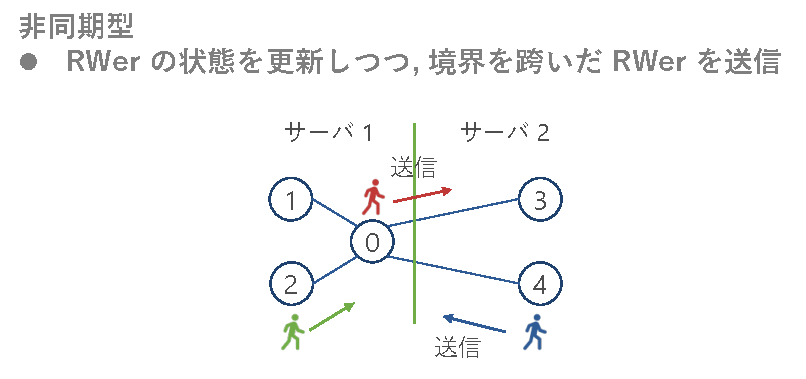
\includegraphics[scale=0.8]{figure/walkercentric_async.pdf}
    \caption{walker centric モデル (非同期型) の概要}
    \label{walker centric モデル (非同期型) の概要}
\end{figure}

次に, 提案手法は RWer の送受信に UDP 通信を採用する. UDP 通信では, たとえ RTT・パケットロス率が高かったとしてもスループットがほとんど低下しない. そのため, 地理的分散環境下における RWer の送受信には UDP 通信が適している. UDP 通信のデメリットはパケットロスが発生することであるが, RW の独立性により, RWer の損失のデメリットは少ない. 図 \ref{局所的に RWer が損失したときの PPR 演算の精度} に局所的に RWer が損失したときの Personalized PageRank (PPR) 演算の精度を示す. PPR とは, ある始点から始めた RW における各頂点の滞在確率を表している. この実験では LiveJournal のデータセット\cite{snapnets} のグラフを 5 台のサーバで分散管理し, ランダムな開始頂点から 50000 回の RW を実行することで RWer の経路情報から PPR を計算した. ここで, サーバ 1, 2, 3, 4 からサーバ 5 への RWer の送信の $x\%$ (図 \ref{局所的に RWer が損失したときの PPR 演算の精度} の横軸) を意図的に落とすことで, RWer が局所的に損失するシミュレーションを行った. PPR 演算精度を NDCG と呼ばれる指標で算出し, ランダムな開始頂点 1000 個分の平均を 図 \ref{局所的に RWer が損失したときの PPR 演算の精度} の縦軸に設定した. NDCG は 1 に近づくほど精度が高くなり, 0.999 程度あれば真値とほとんど等しい. NDCG が 0.999 を下回るのは意図的に落とす確率が 15 $\%$ のときであるため, RWer の損失が RW を利用したアプリケーションへ及ぼす影響は少ないことがわかる. 

UDP 通信の他にも QUIC と呼ばれる UDP 通信を用いて高速化しつつ TCP 通信のような通信の信頼性を提供するトランスポート層のプロトコルがある. UDP 通信に対する QUIC のメリットは, 認証・暗号化による安全性, そして再送制御による信頼性である. しかし本研究において, 安全性は現時点では不必要であり, 図 \ref{局所的に RWer が損失したときの PPR 演算の精度} のようにパケットロスの影響が少ないため再送制御も不必要である. そのため本研究では QUIC ではなく UDP 通信を採用した. 

また, 提案手法は終了した RWer の経路再利用により, 通信量を削減する. 詳細は \ref{Random Walker の経路再利用} にて述べる. 

\begin{figure}[t]
    \centering
    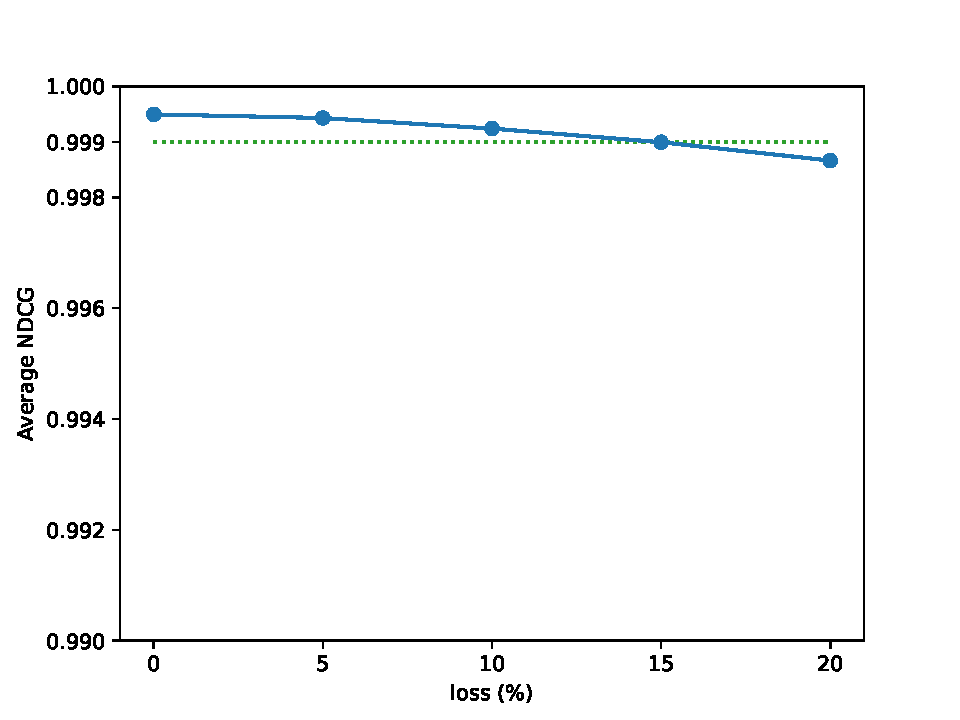
\includegraphics[scale=0.7]{figure/eva_drop.pdf}
    \caption{局所的に RWer が損失したときの PPR 演算の精度}
    \label{局所的に RWer が損失したときの PPR 演算の精度}
\end{figure}

\section{Random Walker の構成}\label{Random Walker の構成}

本節では提案手法における RWer の構成について述べる. 表 \ref{RWer の構成} に RWer の構成を示す. $ver\_id\_$ はバージョンとメッセージ ID を含んでおり, メッセージ ID によって, 生存している RWer, 終了した RWer, 複数の RWer が入っているパケットを識別する. この $ver\_id\_$ はメッセージの送受信におけるパケットにも付与するがその詳細については \ref{実装} 節で述べる. $flag\_$ では RW 処理をする上で必要となる情報をフラグとして保持する. 1 hop 前で通信が発生したかを保持しておくことで, その遷移先で経路情報における通信発生フラグを立てることができる. また, $next\_index\_$ に値が入っているかを保持しておくことで, \ref{Random Walker の経路再利用} 節で説明する送信先での index による遷移を行うことができる. そして全体を通して通信が発生したかを保持しておくことで, 終了した RWer を他のサーバに送信するかどうかを判断することができる. $RWer\_size\_$ は RWer 単体のメモリサイズを保持する. これはメッセージ送信時の複数の RWer をまとめる際に必要となる. $RWer\_id\_$ は RWer の識別 ID である. $RWer\_life\_$ は RW 演算における残り hop 数を保持する. 提案手法では RWer 生成時に経路長を先に計算する. 例えば各遷移ごとで確率 $\alpha (< 1)$ で終了する RW 演算であれば, $0 < r < 1$ の乱数を $r < \alpha$ となるまで生成し, その生成回数を経路長とする. この $RWer\_life\_$ はサーバ上で RWer の構造体を生成する際, 可変長配列である $path\_$ のメモリ確保に使用される. $path\_length\_at\_current\_host\_$ は RWer の現在の同一ホスト内における経路長を保持する. これは $path\_$ における現在ホスト情報の位置を特定する際に使用される. $next\_index\_$ は通信が発生したときの次の遷移先 index を示す. これは RWer の経路再利用機能で使用される. 

\begin{table}[t]
    \caption{RWer の構成}
    \label{RWer の構成}
    \centering
    \begin{tabular}{ccc}
        \hline
        名称  &  サイズ  &  内容 \\
        \hline \hline
        $ver\_id\_$  &  8 bit  &  バージョン: 4 bit, メッセージ ID: 4 bit \\
        \hline
        $flag\_$  &  8 bit  & 
        \begin{tabular}{c} 1 hop 前で通信が発生したか: 1 bit, \\$next\_index\_$ に値が入っているか: 1 bit, \\全体を通して通信が発生したか: 1 bit, \\予備: 5 bit 
        \end{tabular}\\
        \hline
        $RWer\_size\_$  &  16 bit  &  RWer 単体のメモリサイズ \\
        \hline
        $RWer\_id\_$  &  32 bit  &  RWer の識別 ID \\
        \hline
        $RWer\_life\_$  &  16 bit  &  RWer の残り歩数  \\
        \hline
        $path\_length\_at\_current\_host\_$  &  16 bit  &  RWer の現在の同一ホスト内の経路長  \\
        \hline
        $reserved\_$  &  32 bit  &  予備  \\
        \hline
        $next\_index\_$  &  64 bit  &  通信が発生したときの次の遷移先 index \\
        \hline
        $path\_$  &  64 bit の可変長配列  &  経路情報  \\
        \hline
    \end{tabular}
\end{table}

図 \ref{経路情報の構成} に $path\_$ (経路情報) の構成を示す. $path\_$ は, ホスト情報 (64 bit), 頂点情報 (64 bit $\times$ 4), 頂点情報, ... , ホスト情報, 頂点情報, ... のように頂点情報をホストごとにグループ化する. これにより各頂点情報にその頂点を保有するホストの情報を入れる必要がなくなり, サイズを削減することができる. ホスト情報の構成は, HostID (48 bit), 同一 HostID 内の経路長 (15 bit), 通信が発生したかどうかのフラグ (1 bit) である. 同一 HostID 内の経路長は経路情報を前方から探索していく際に必要となる. 通信が発生したかどうかのフラグは, 経路再利用による通信スキップが発生しなかった場合の判定に利用できる. 頂点情報の構成は, 頂点 ID (64 bit), 次数 (64 bit), $u \rightarrow v$ の index (64 bit), $v \rightarrow u$ の index (64 bit) である. $u \rightarrow v$ の index はひとつ前の頂点から見た今の頂点の index 情報であり, $v \rightarrow u$ の index は今の頂点から見たひとつ前の頂点の index 情報である. 逆方向の index 情報を保持しておくことで, 無向グラフにおける逆向きの経路情報も再利用することができる. 次数情報は経路再利用時に使用されるため頂点情報に含まれている. 

\begin{figure}[t]
    \centering
    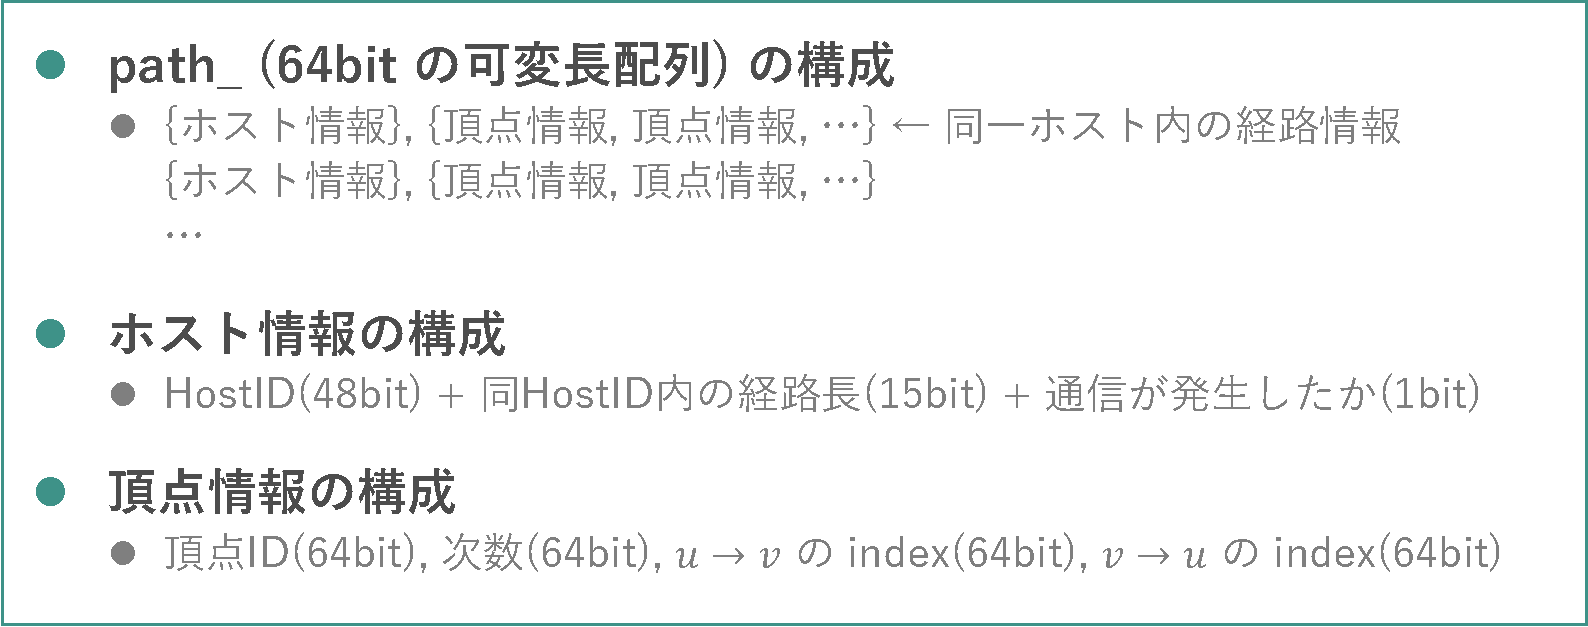
\includegraphics[scale=0.5]{figure/path.pdf}
    \caption{経路情報の構成}
    \label{経路情報の構成}
\end{figure}

\section{Random Walker の経路再利用}\label{Random Walker の経路再利用}



\section{実装}\label{実装}